\section{Model-free Reinforcement Learning}
Can view TD-learning as SGD on the squared loss $\ell(\vtheta; x, r, x') \defeq \frac{1}{2}\parentheses*{r + \gamma \old{\vtheta}(x') - \vtheta(x)}^2$. \\
\textbf{Parametric value function approximation}: To scale to large state spaces, learn approximation
of (action) value function $\V{\vx; \vtheta}$ or $\Q{\vx}{\va; \vtheta}$. E.g., the parameters $\vtheta$ of a neural network.
\begin{framed}
    \textbf{Q-learning with function approximation}: In state $\vx$, pick action $a$; Observe $\vx'$, reward $r$. Update $\vtheta \gets \vtheta + \alpha_t \delta_\mathrm{B} \vphi(\vx, \va)$, where $\delta_\mathrm{B} \defeq r + \gamma \max_{\vap \in \spA} \Q*{\vxp}{\vap; \old{\vtheta}} - \Q*{\vx}{\va; \vtheta}$.
\end{framed}
\textbf{DQN}: Target network updated infrequently. \\
Q, DQN suffer maximization bias $\Rightarrow$ Double DQN: pick optimal $a$ wrt. \textit{new} network.
\begin{framed}
    Given a policy $\pi$, the \textbf{advantage function} is $\a[\pi]{\vx}{\va} \defeq \q[\pi]{\vx}{\va} - \v[\pi]{\vx} = \q[\pi]{\vx}{\va} - \E[\vap \sim \pi(\vx)]{\q[\pi]{\vx}{\vap}}$
\end{framed}
$\text{$\pi$ is optimal} \iff \forall \vx \in \spX, \va \in \spA : \a[\pi]{\vx}{\va} \leq 0$
\begin{framed}
    \textbf{Policy value function} $=$ disc. payoff of $\pi$: \\
    $\j{\pi} \defeq \E[\pi]{G_0} = \E[\pi]{\sum_{t=0}^\infty \gamma^t R_t}$, \\
     $\j{\pi}[T] \defeq \E[\pi]{G_{0:T}} = \E[\pi]{\sum_{t=0}^{T-1} \gamma^t R_t}$ (bounded). \\
    Abbreviate $\j{\vvarphi} \defeq \j{\pi_\vvarphi}$
\end{framed}
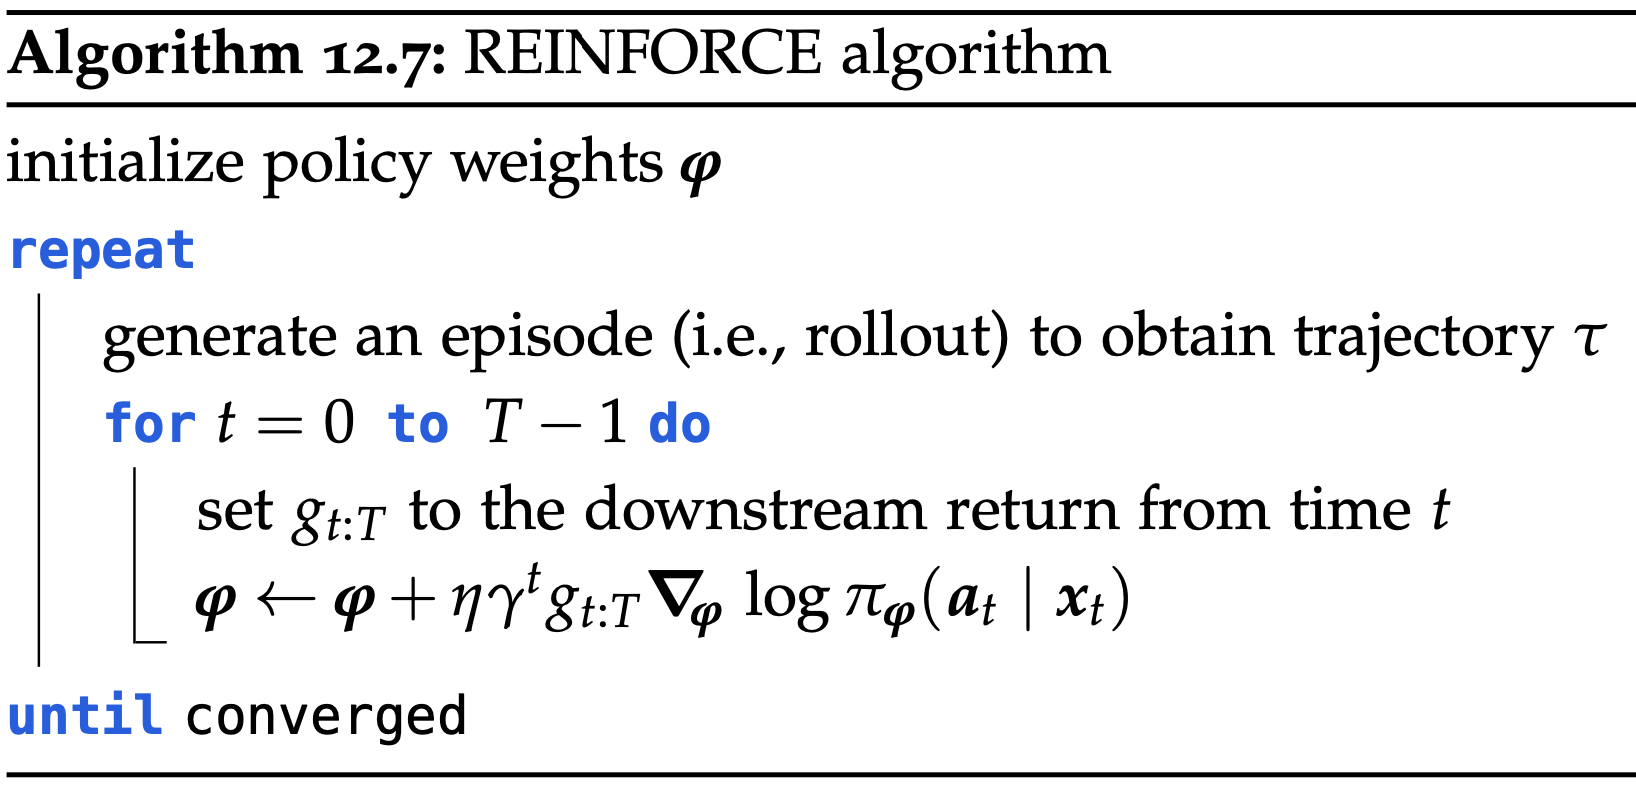
\includegraphics[width=0.9\linewidth]{images/REINFORCE.png}
On-policy, model-free, local minima. \\
For large (cont.) action spaces.
\begin{framed}
  \textbf{Actor-Critic methods} \\
  \textbf{Actor}: parameterized policy, $\pi(\va \mid \vx; \vvarphi) \eqdef \pi_\vvarphi$ \\
  \textbf{Critic}: value function approximation \\
   $\q[\pi_\vvarphi]{\vx}{\va} \approx \Q[\pi_\vvarphi]{\vx}{\va; \vtheta}$ abbreviate $\fnQ[\pi_\vvarphi]$ by $\fnQ$.
\end{framed}
Use gradient approximation: 
{\tiny$\grad_\vvarphi \J{\vvarphi} \approx \sum_{t=0}^\infty\E[(\vx_t,\va_t) \sim \pi_\vvarphi]{\gamma^t \Q{\vx_t}{\va_t; \vtheta} \grad_\vvarphi \log \pi_\vvarphi(\va_t \mid \vx_t)}$}
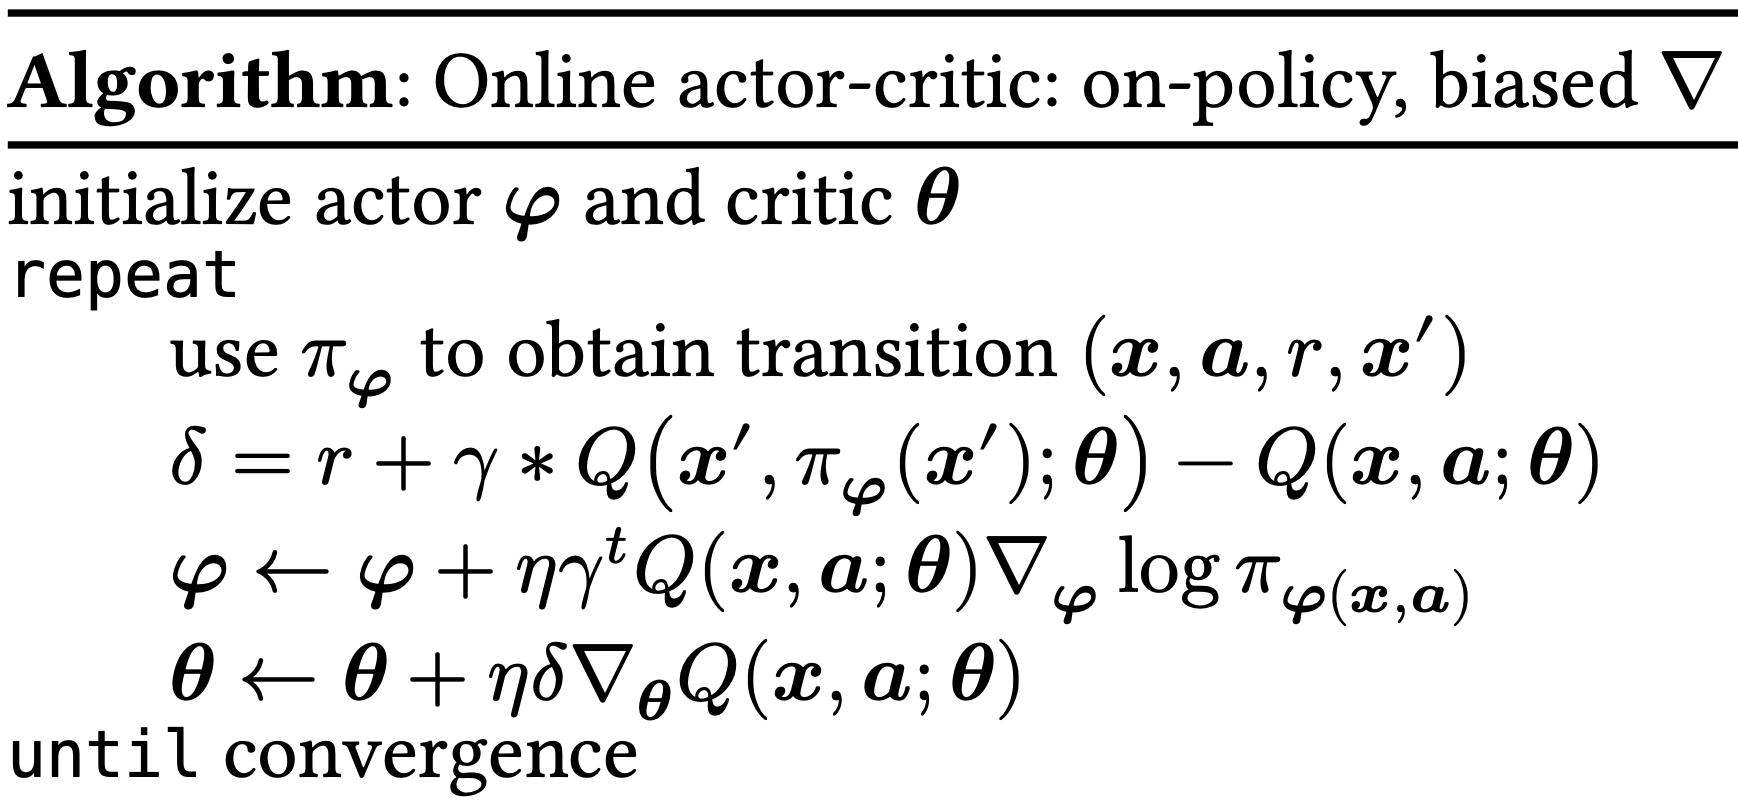
\includegraphics[width=0.8\linewidth, trim={0 0 1cm 0}]{images/Online_actor_critic.png}
A2C: bootstrapped advantage estimate. \\
\textbf{Off-policy Actor-Critic}: DDPG (add noise), TD3 (2 critics), SAC (entropy maximization). \\
Feedback learning: RLHF learns reward model and policy; DPO learns policy directly.